\begin{frame}
  \frametitle{Some NDL simulation runs}

  \centering
  \only<beamer:1-7| handout:0>{\ungap[2]}%
  \only<beamer:1| handout:0>{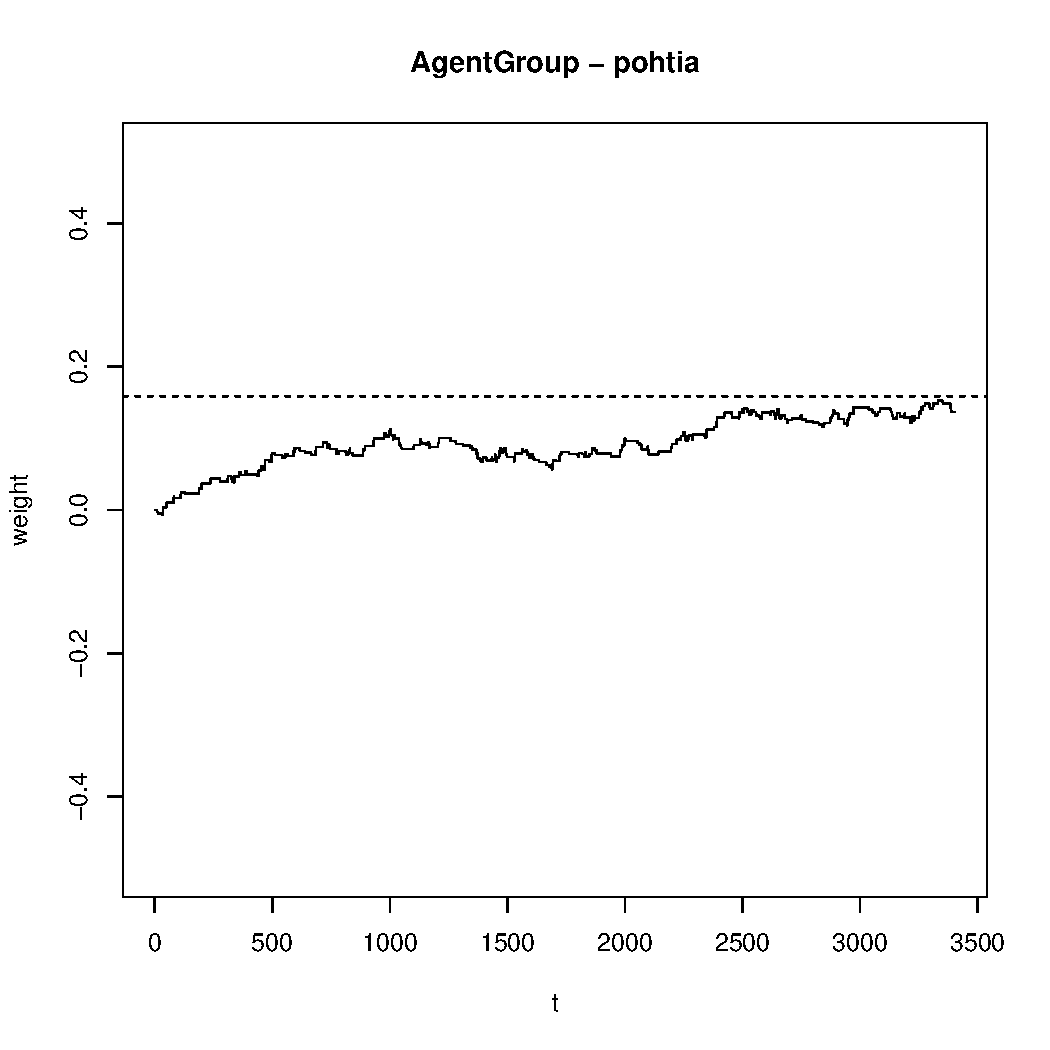
\includegraphics[width=7.5cm]{{{img/think.qitl2.AgentGroup_pohtia_RW_vs_D}}}}%
  \only<beamer:2| handout:0>{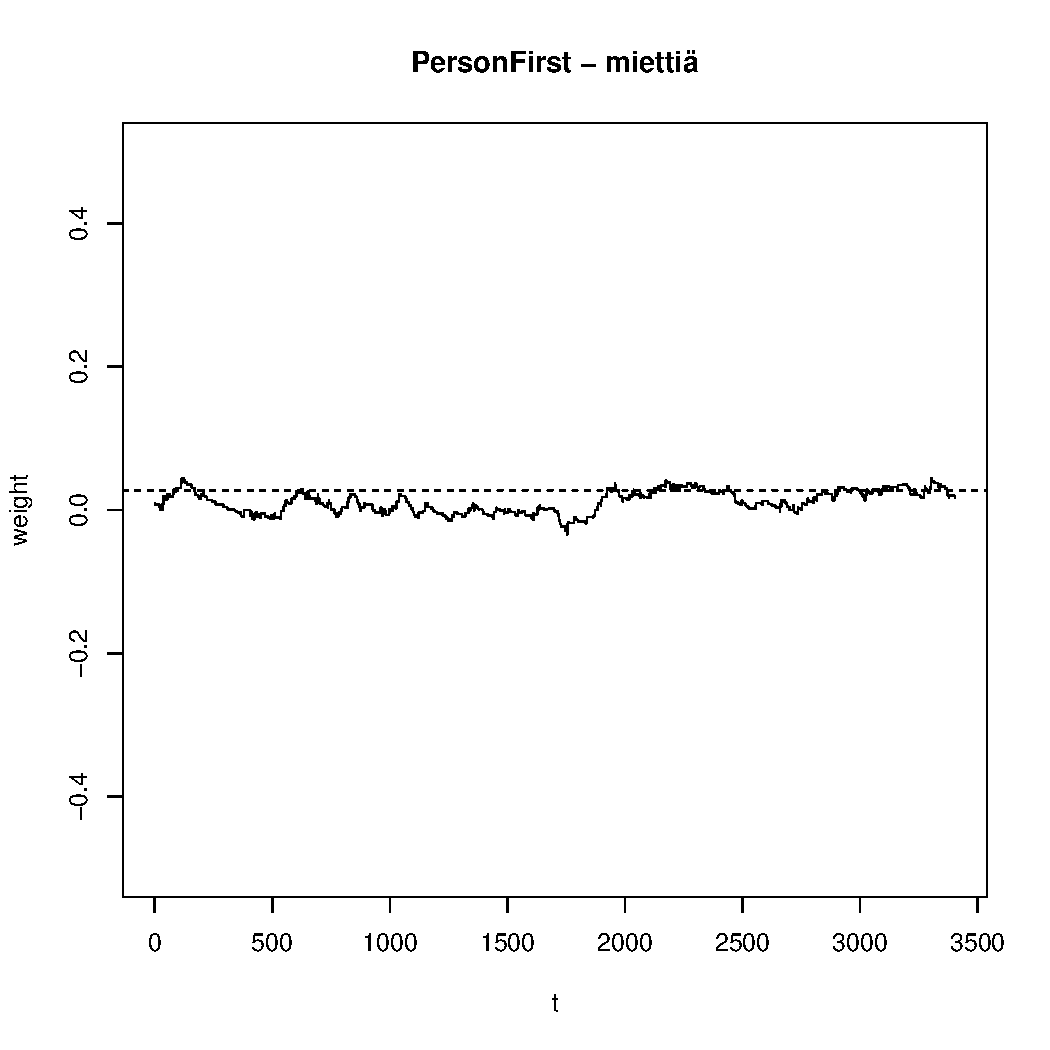
\includegraphics[width=7.5cm]{{{img/think.qitl2.PersonFirst_miettia_RW_vs_D}}}}%
  \only<beamer:3| handout:0>{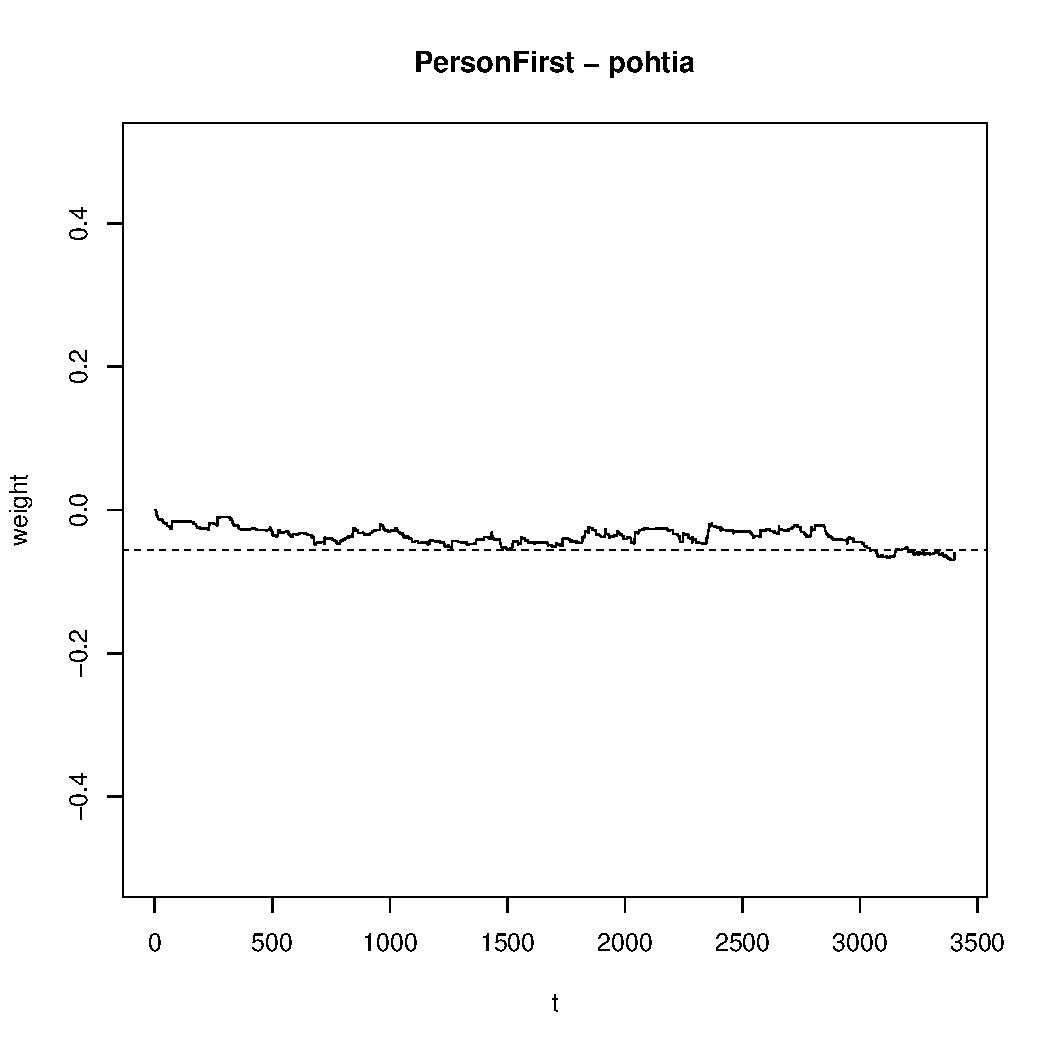
\includegraphics[width=7.5cm]{{{img/think.qitl2.PersonFirst_pohtia_RW_vs_D}}}}%
  \only<beamer:4| handout:0>{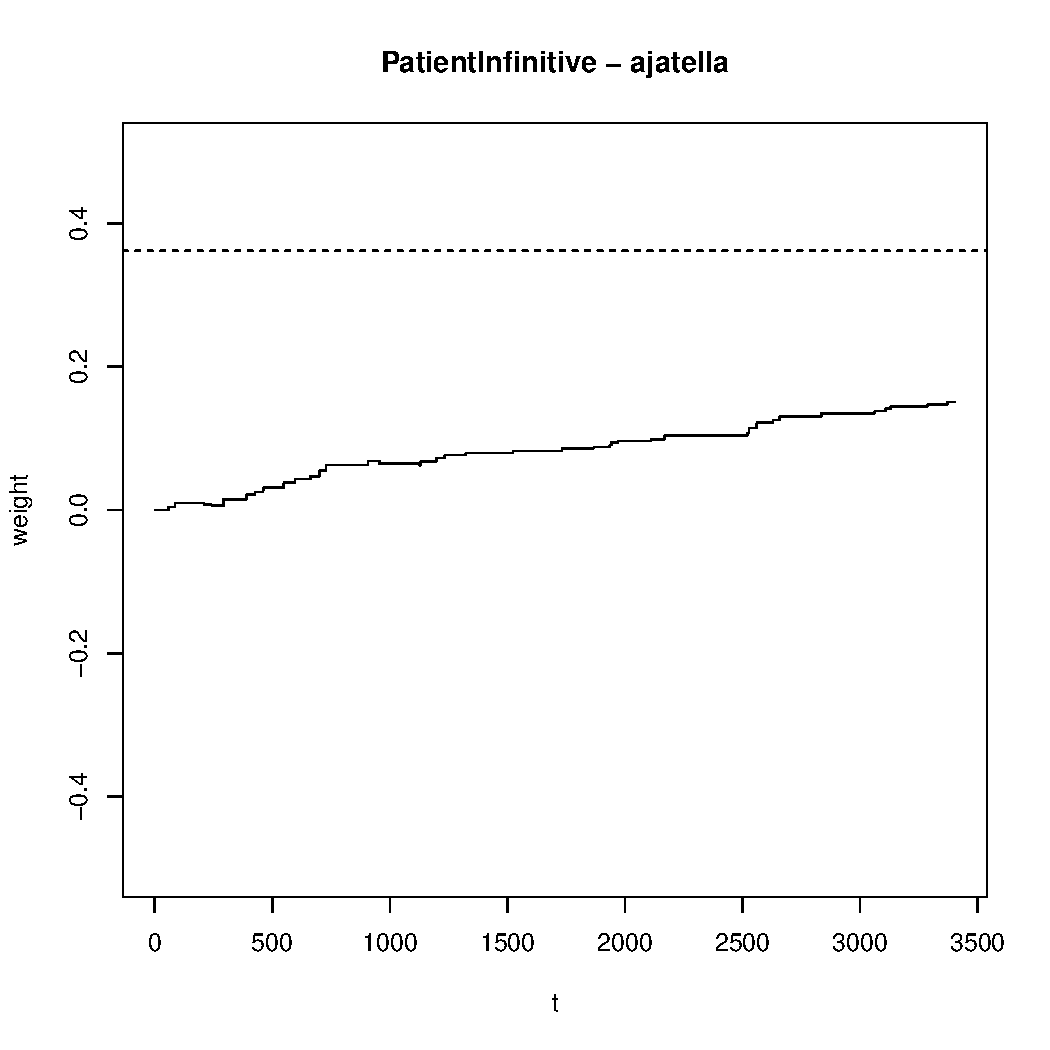
\includegraphics[width=7.5cm]{{{img/think.qitl2.PatientInfinitive_ajatella_RW_vs_D}}}}%
  \only<beamer:5| handout:0>{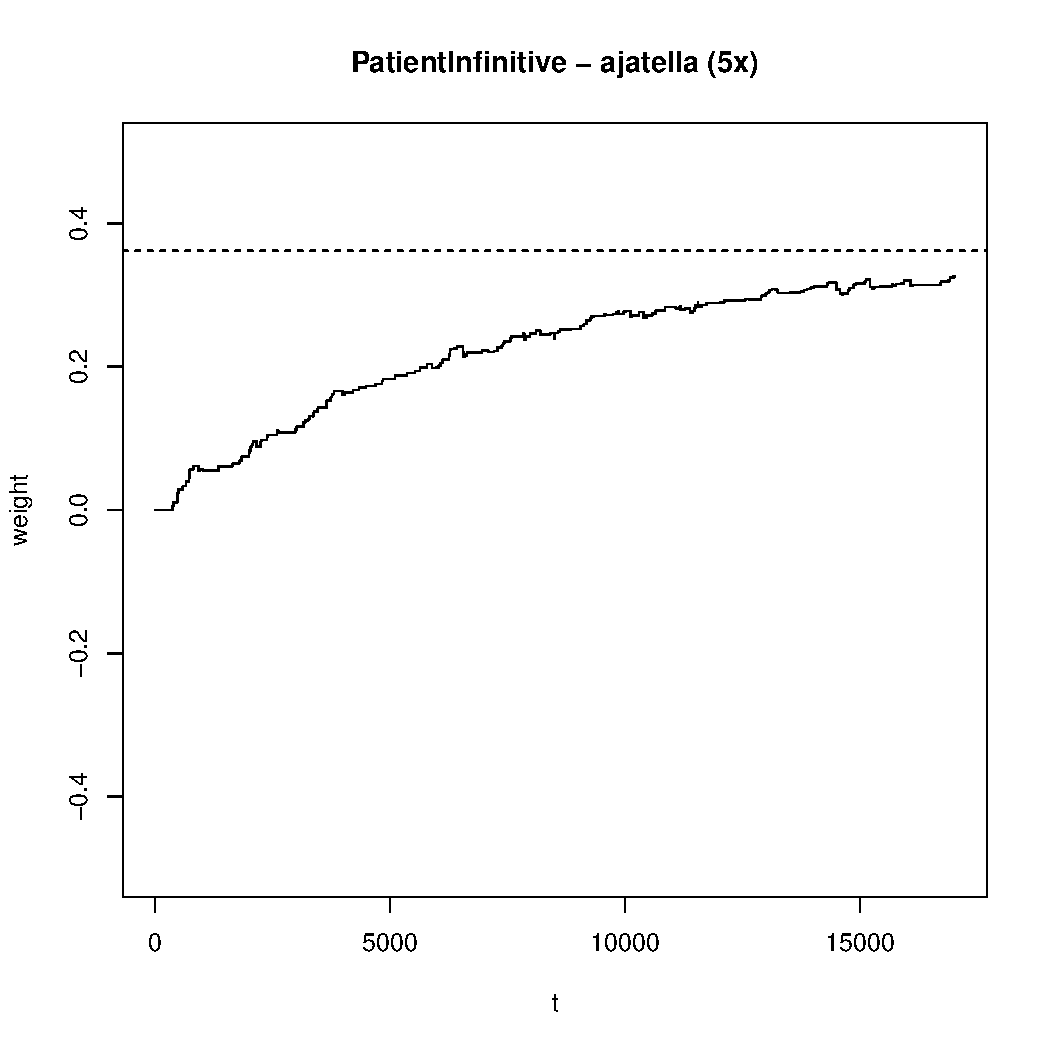
\includegraphics[width=7.5cm]{{{img/think.qitl2.PatientInfinitive_ajatella_RW_vs_Dx5}}}}%
  \only<beamer:6| handout:0>{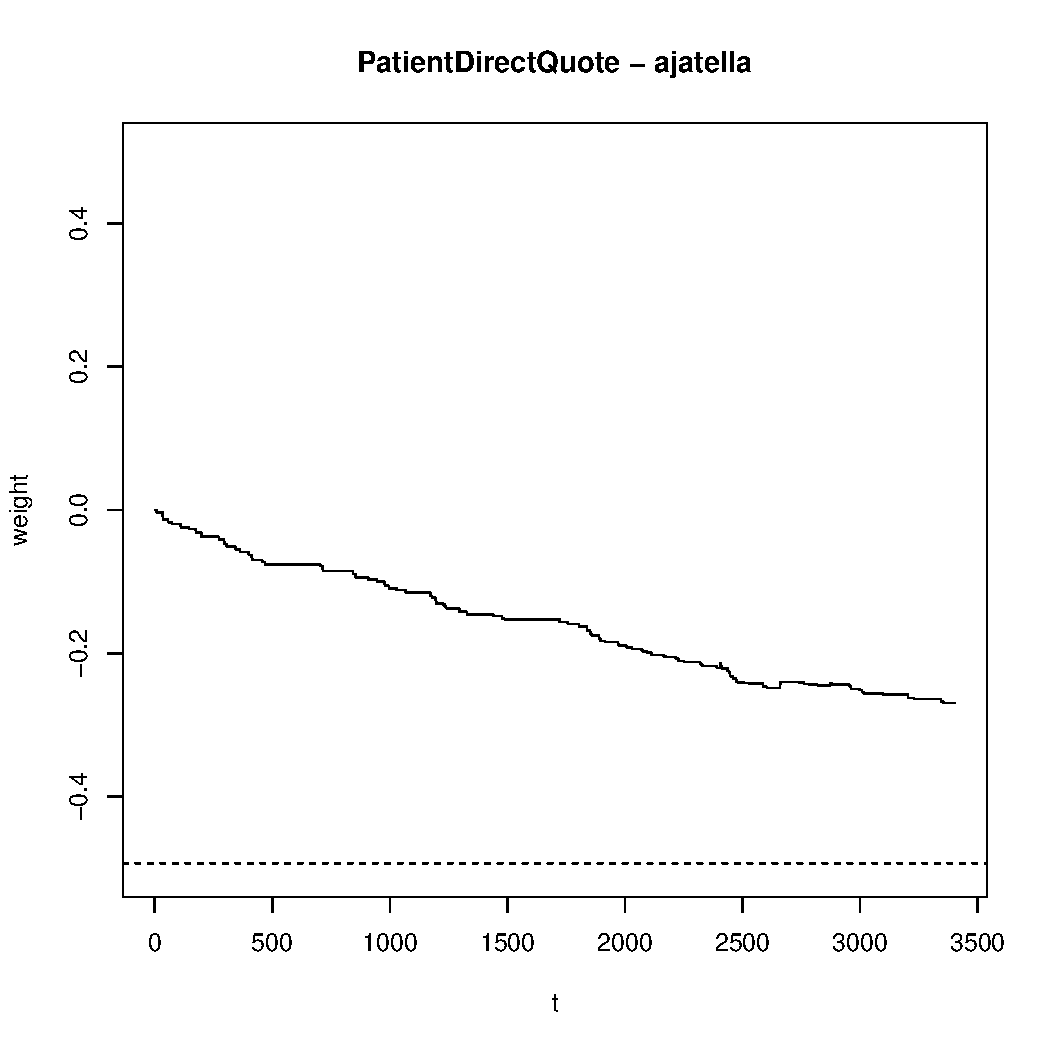
\includegraphics[width=7.5cm]{{{img/think.qitl2.PatientDirectQuote_ajatella_RW_vs_D}}}}%
  \only<beamer:7| handout:0>{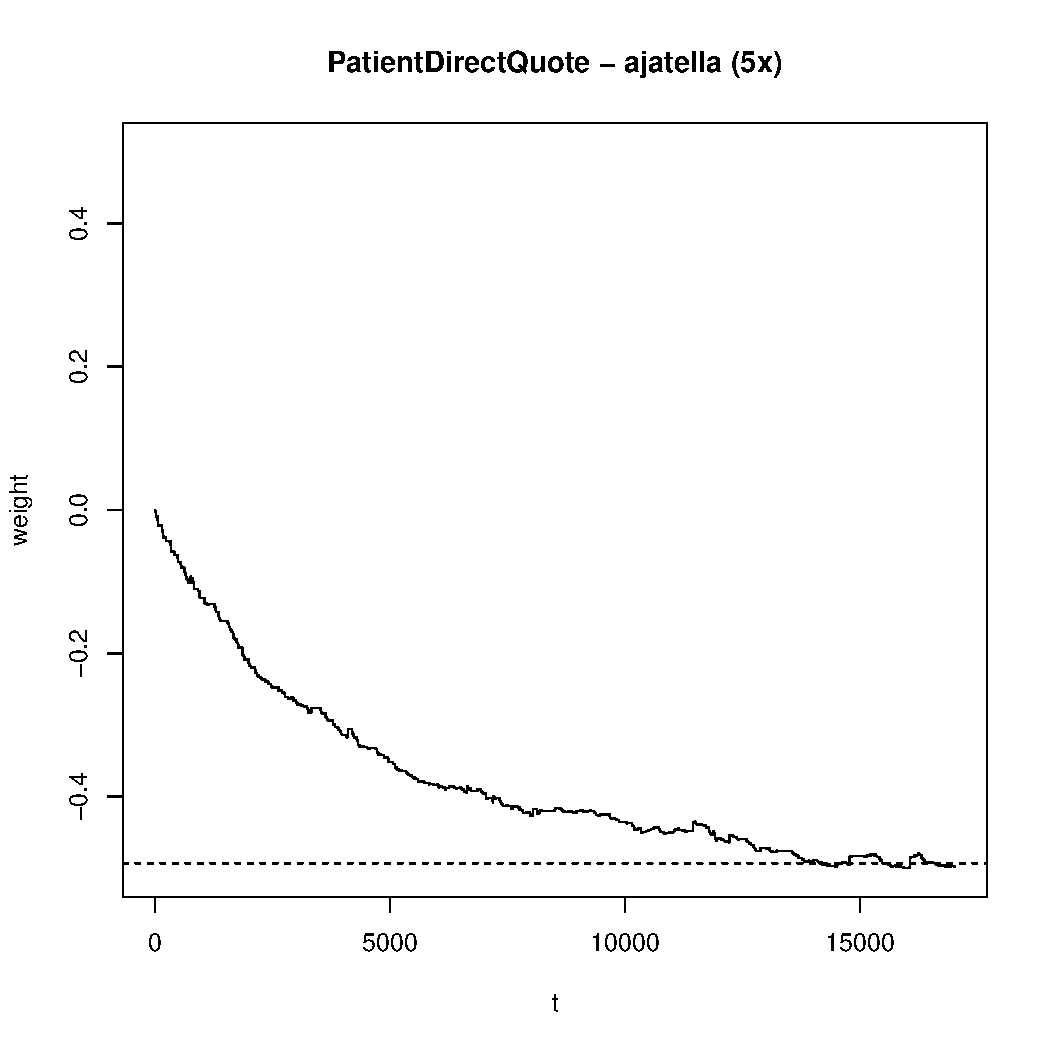
\includegraphics[width=7.5cm]{{{img/think.qitl2.PatientDirectQuote_ajatella_RW_vs_Dx5}}}}%
  \only<beamer:1-7| handout:0>{\\ \ungap[.5]\color{secondary}}%
  \only<beamer:1| handout:0>{moderate positive association \so convergence}%
  \only<beamer:2| handout:0>{equivocal association \so convergence}%
  \only<beamer:3| handout:0>{equivocal association \so convergence}%
  \only<beamer:4| handout:0>{near-perfect positive association \so non-convergence with $1\times$ data}%
  \only<beamer:5| handout:0>{near-perfect positive association \so convergence with $5\times$ data}%
  \only<beamer:6| handout:0>{near-perfect negative association \so non-convergence with $1\times$ data}%
  \only<beamer:7| handout:0>{near-perfect negative association \so convergence with $5\times$ data}%
  \only<beamer:0| handout:1>{%
    \begin{tabular}{ccc}
      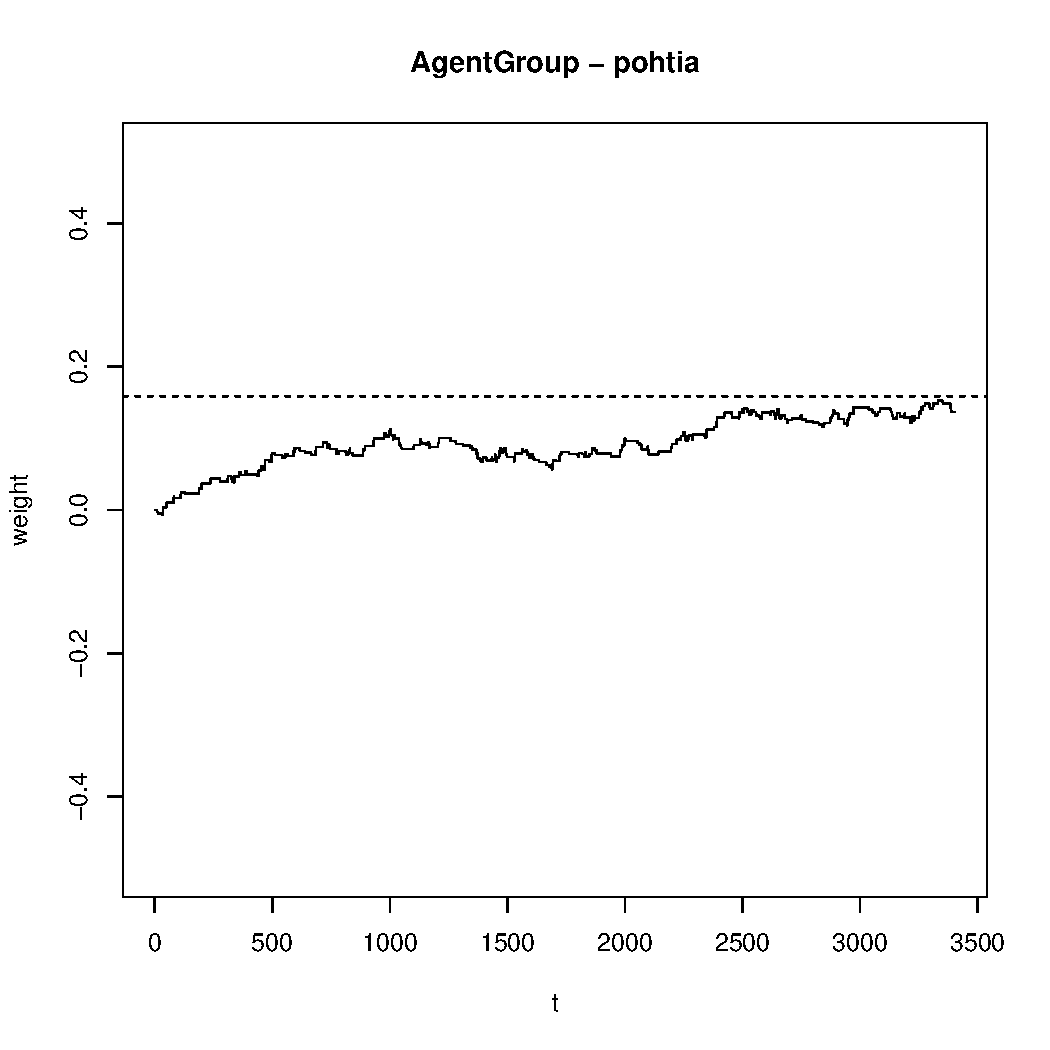
\includegraphics[width=3.5cm]{{{img/think.qitl2.AgentGroup_pohtia_RW_vs_D}}} &
      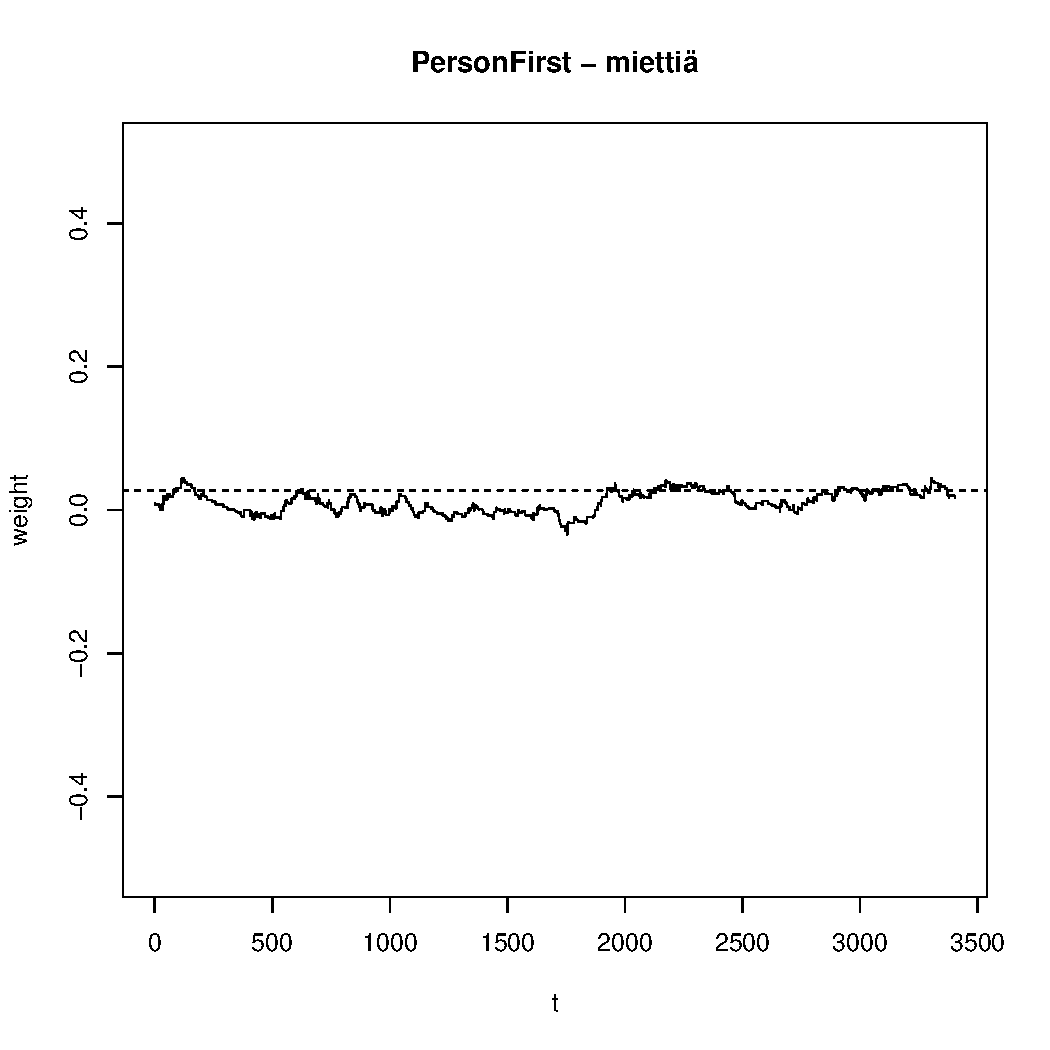
\includegraphics[width=3.5cm]{{{img/think.qitl2.PersonFirst_miettia_RW_vs_D}}} &
      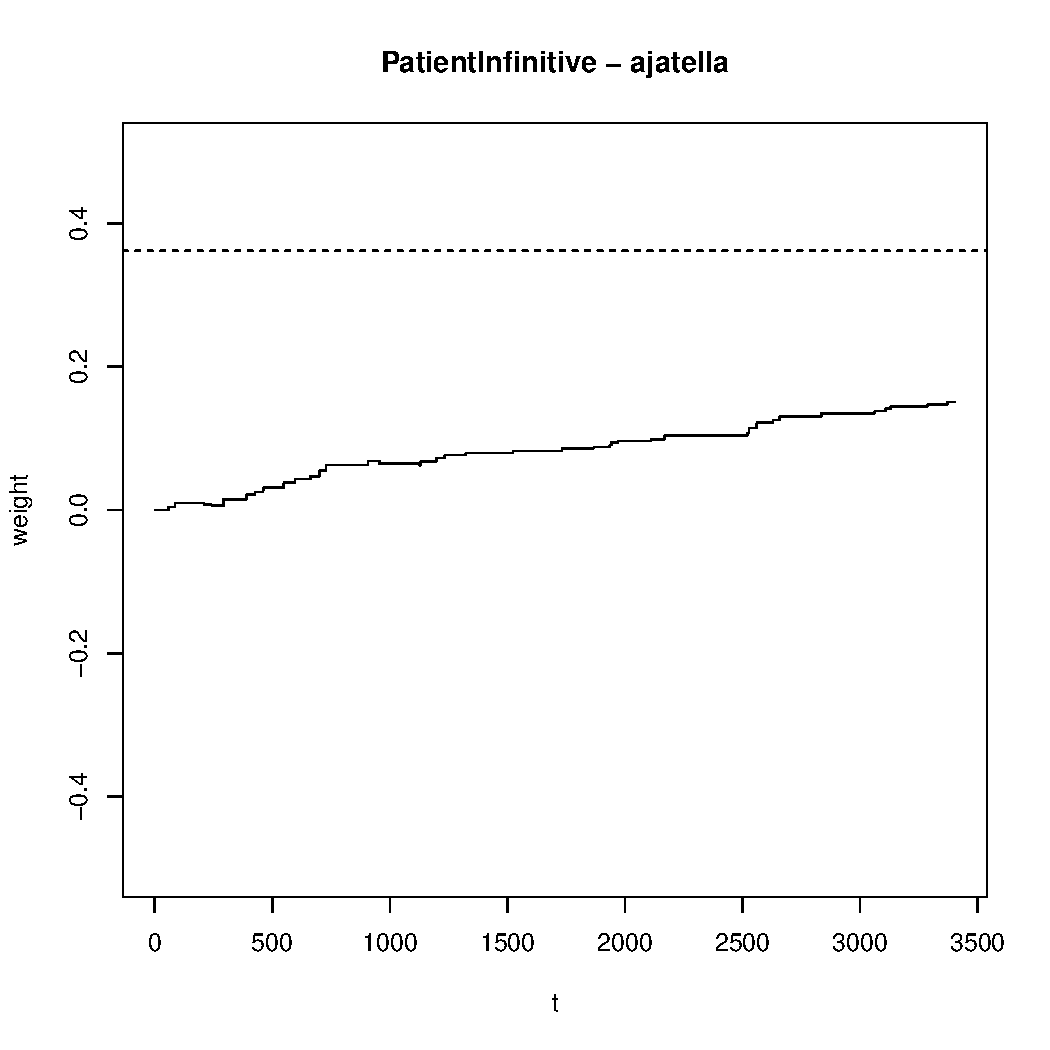
\includegraphics[width=3.5cm]{{{img/think.qitl2.PatientInfinitive_ajatella_RW_vs_D}}} \\
      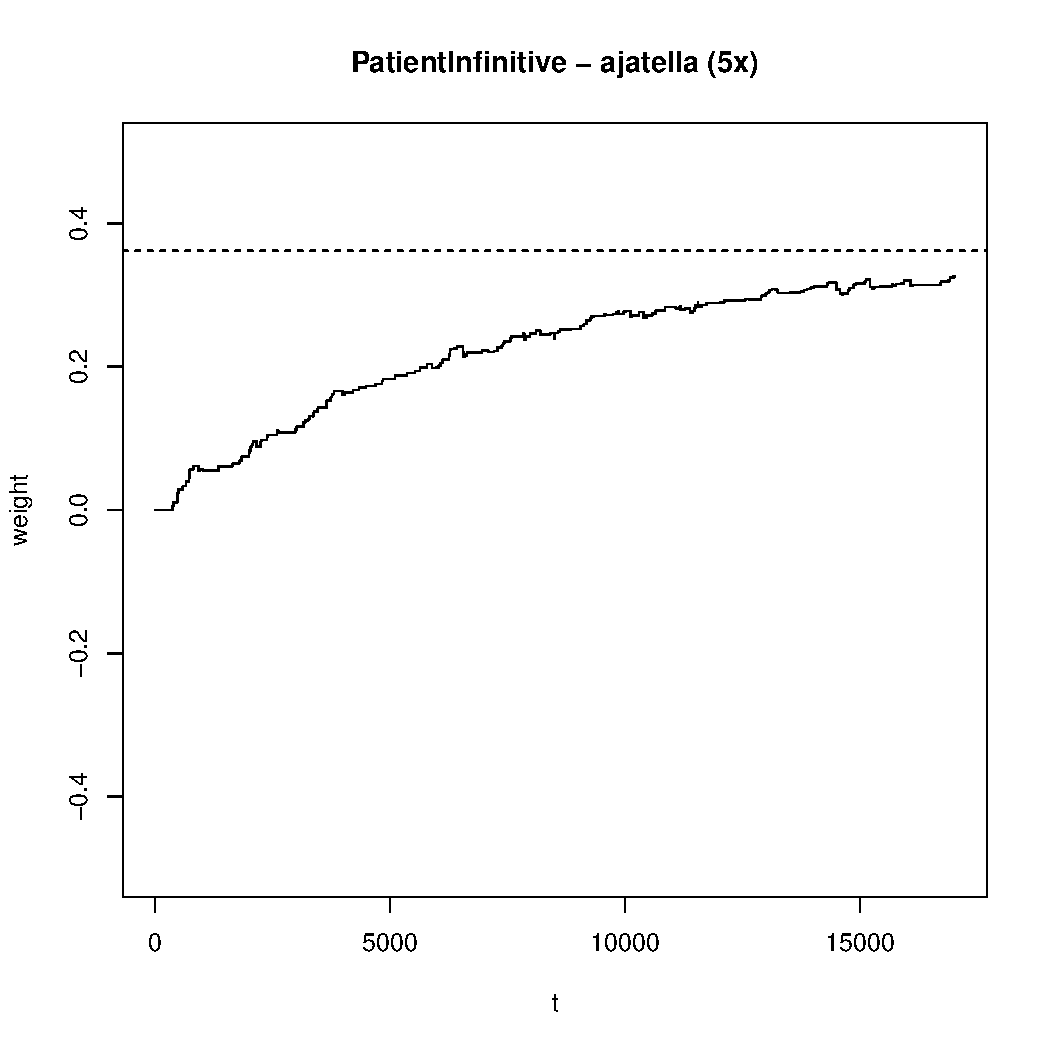
\includegraphics[width=3.5cm]{{{img/think.qitl2.PatientInfinitive_ajatella_RW_vs_Dx5}}} &
      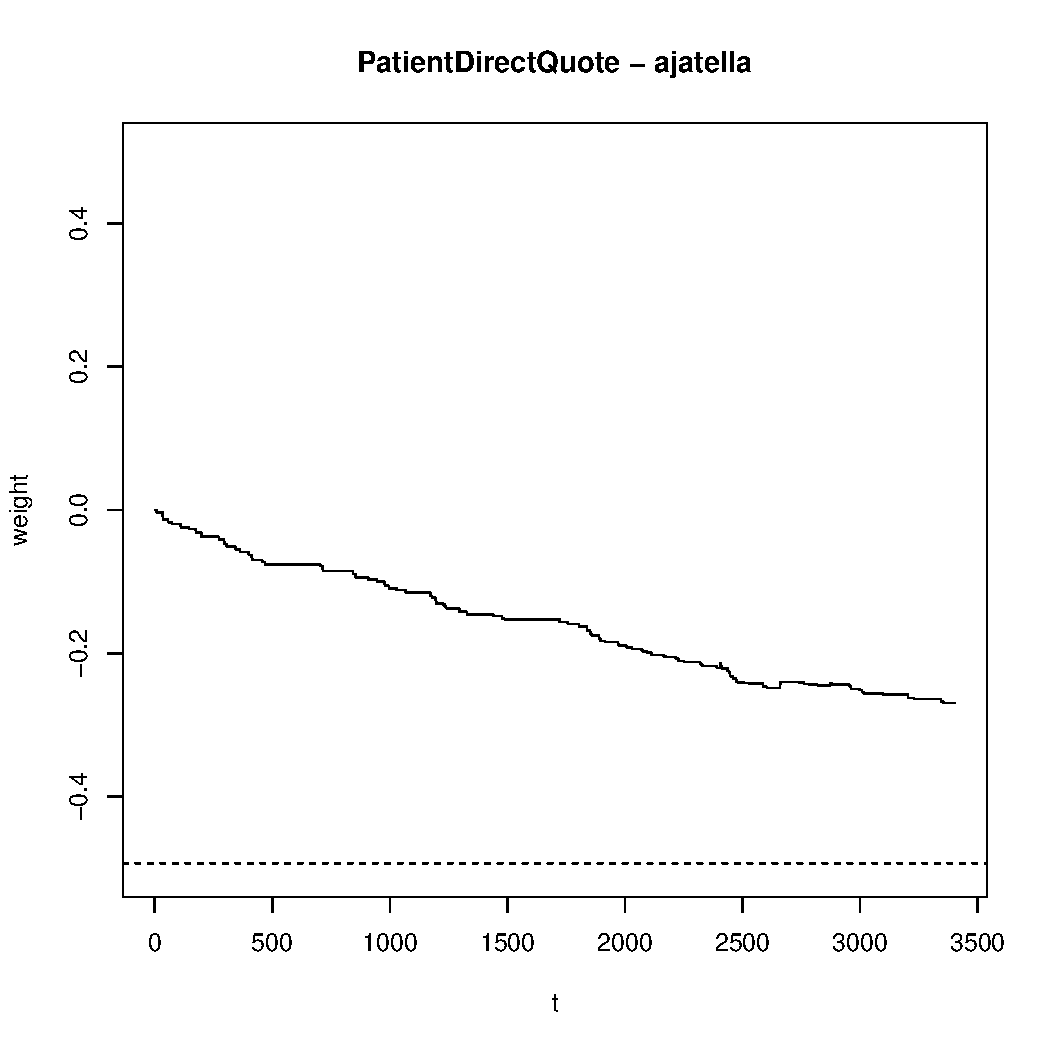
\includegraphics[width=3.5cm]{{{img/think.qitl2.PatientDirectQuote_ajatella_RW_vs_D}}} &
      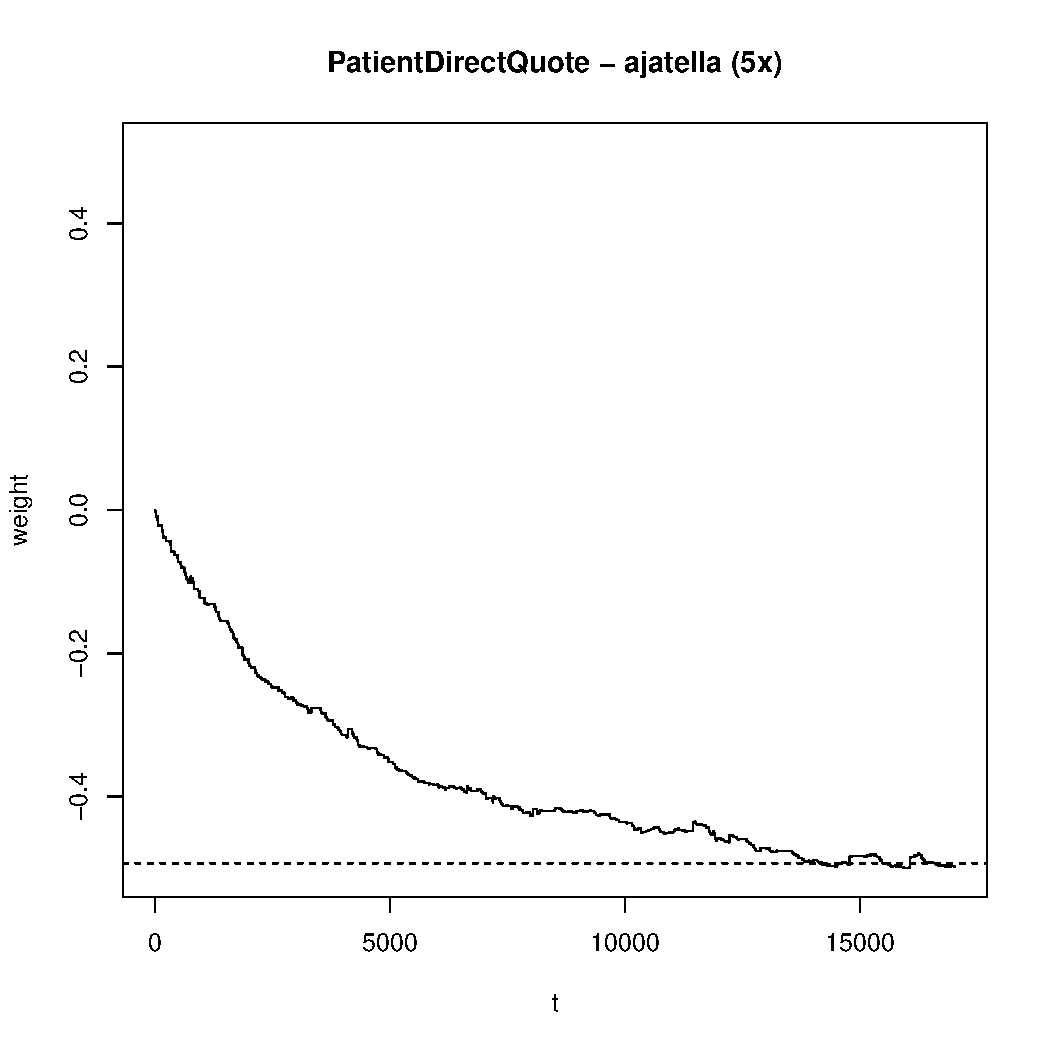
\includegraphics[width=3.5cm]{{{img/think.qitl2.PatientDirectQuote_ajatella_RW_vs_Dx5}}}
    \end{tabular}    
  }%
\end{frame}


\begin{frame}
  \frametitle{Convergence \vs non-convergence -- artificial data}

  \begin{center}
    \begin{tabular}{ l r r >{\color{secondary}}r }
      \toprule
      word form & frequency &   outcomes &  \foreground{cues} \\
      \midrule
      hand &       10 &    \counterpoint{hand}\_NIL &   h\_a\_n\_d \\
      hands &       20 & \counterpoint{hand}\_\primary{PLURAL} & h\_a\_n\_d\_s \\
      land &        8 &    land\_NIL &   l\_a\_n\_d \\
      lands &        3 & land\_\primary{PLURAL} & l\_a\_n\_d\_s \\
      and &       35 &     and\_NIL &     a\_n\_d \\
      sad &       18 &     sad\_NIL &     s\_a\_d \\
      as &       35 &      \fourth{as}\_NIL &       a\_s \\
      lad &      102 &     lad\_NIL &     l\_a\_d \\
      lad &       54 &  lad\_\primary{PLURAL} &     l\_a\_d \\
      lass &      134 &    lass\_NIL &   l\_a\_s\_s \\
      \bottomrule
    \end{tabular}
  \end{center}
\end{frame}

\begin{frame}[c]
  \frametitle{Perfect positive association \so convergence}

  \centering
  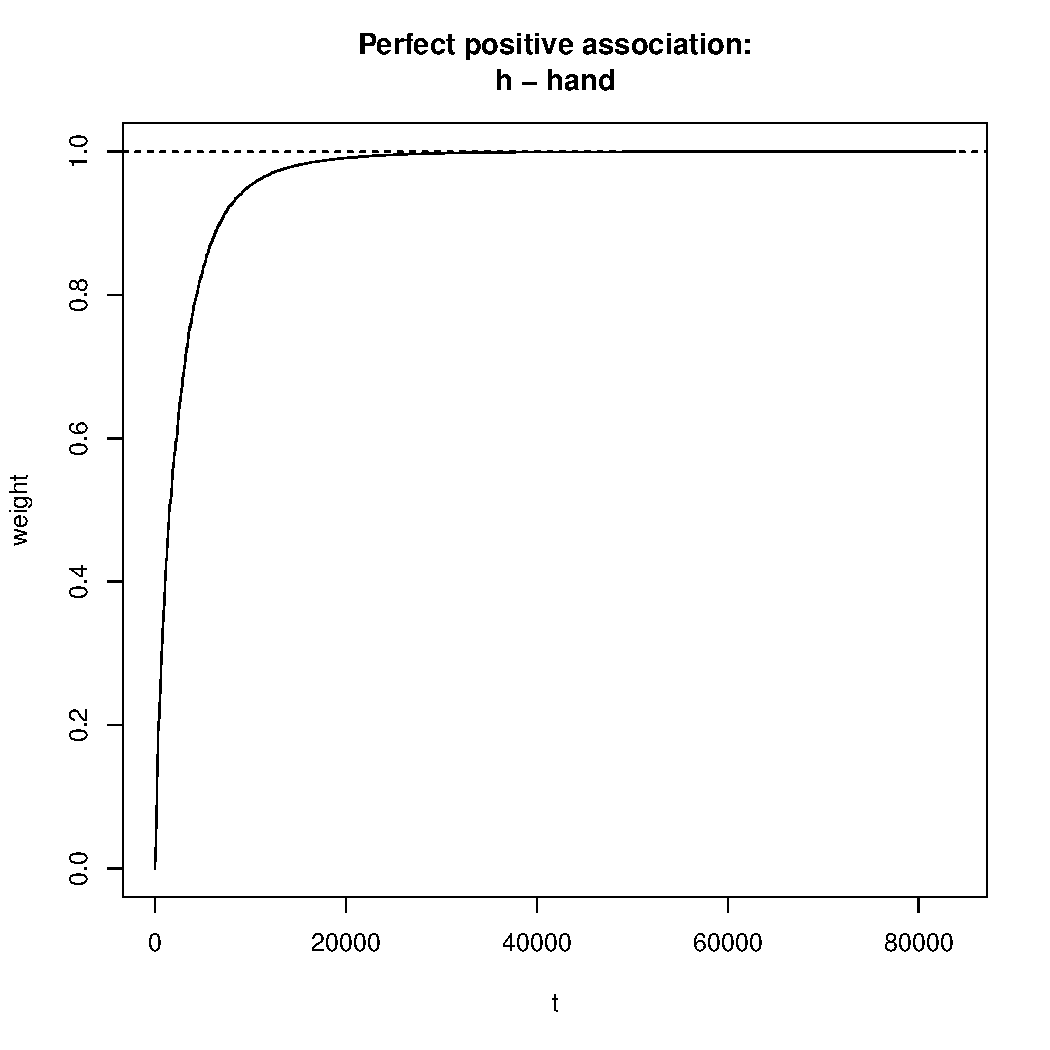
\includegraphics[width=8cm]{{{img/plurals_h_hand}}}
\end{frame}

\begin{frame}[c]
  \frametitle{Moderate positive association \so non-convergence}

  \centering
  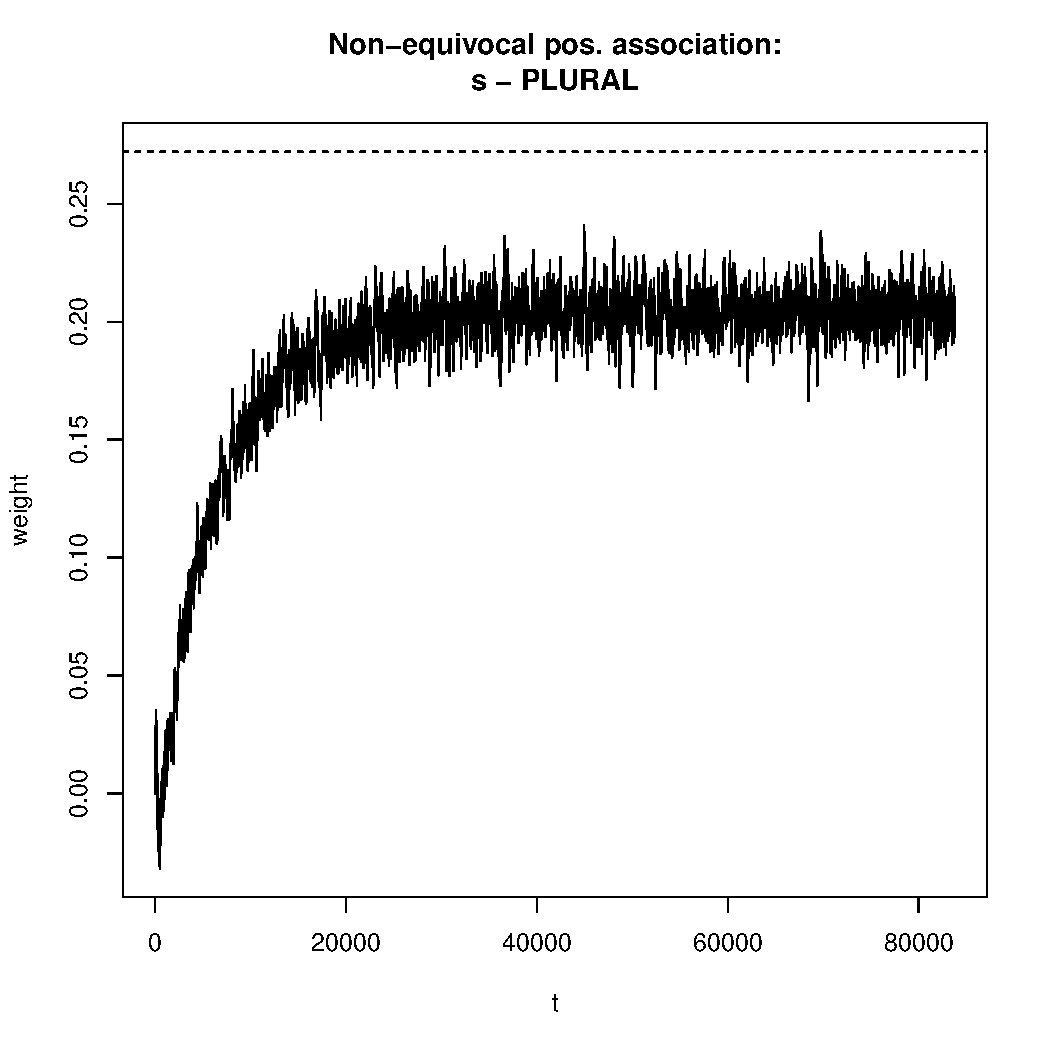
\includegraphics[width=8cm]{{{img/plurals_s_PLURAL}}}
\end{frame}

\begin{frame}[c]
  \frametitle{Perfect positive association \so convergence}

  \centering
  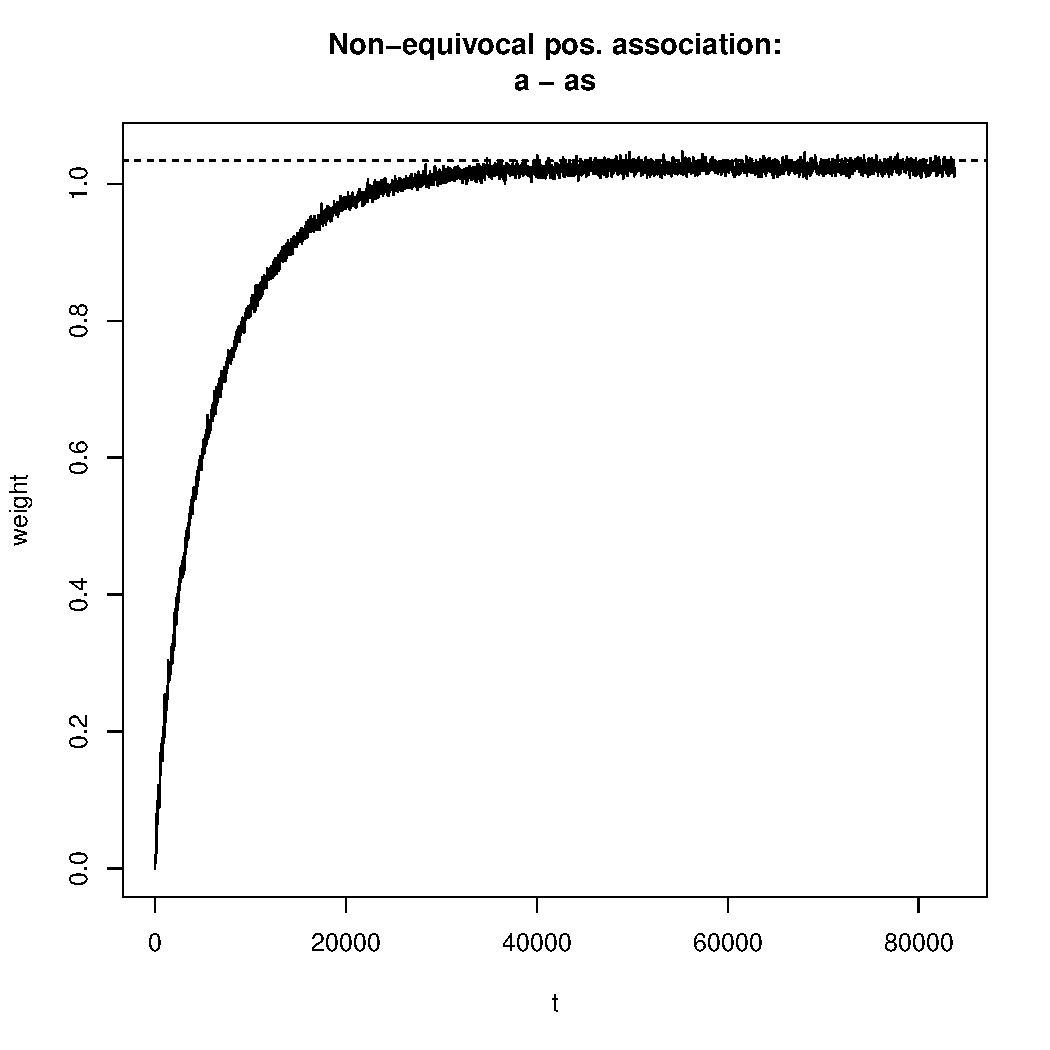
\includegraphics[width=8cm]{{{img/plurals_a_as}}}
\end{frame}

\begin{frame}[c]
  \frametitle{Moderate negative association \so non-convergence}

  \centering
  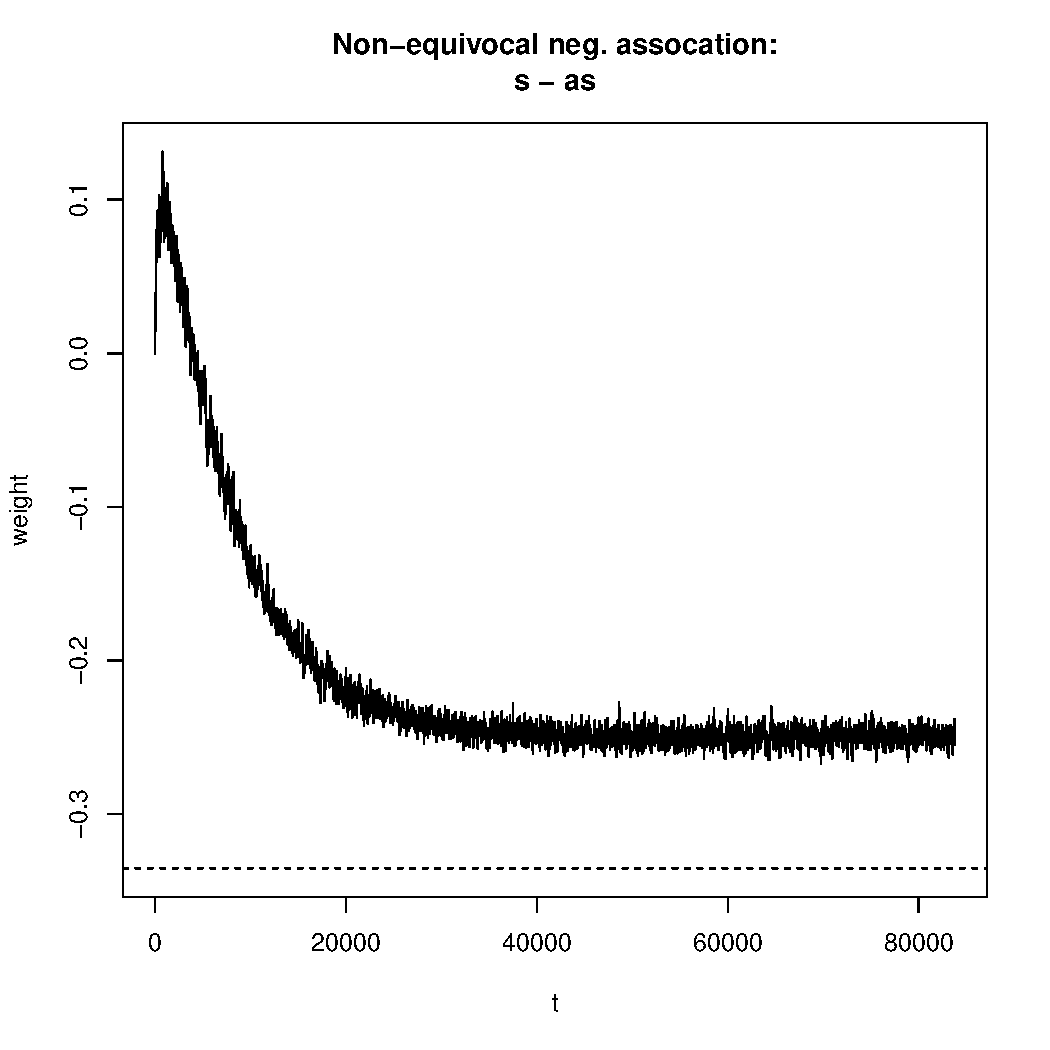
\includegraphics[width=8cm]{{{img/plurals_s_as}}}
\end{frame}

%%% Local Variables: 
%%% mode: latex
%%% TeX-master: "../qitl6_evert_arppe"
%%% End: 
